
In this section, we discuss the graphics capabilities of Matlab.

\section{Matlab: Graphics}\label{sec:Matlab_graphics}

The main commands that we will use in this chapter are\\
\\
\cour{plot}, \cour{subplot},\cour{figure} and \cour{hold} \\
\\
and the customizations\\
\\ 
\cour{xlim}, \cour{ylim}, \cour{xlabel}, \cour{ylabel}, and \cour{title}.\\

Plots in Matlab are created by simply ``connecting the dots.''  This means that you have to provide the actual coordinates of the points $-$ both the $x$ and $y$ coordinates.  It is not enough to simply say plot $y=x^2$, you must give \underline{exactly} which $x$ values you want squared. \\

\index{Matlab Functions!\cour{plot}}
\example{ex_basicplot}{\textbf{Basic Plot}\\

Define:\\
\\
\cour{>> x = [1:10]; y = [4 15 7 17 8 19:23];}\\

Then to plot the corresponding coordinates, connected by line segments, use\\
\\
\cour{plot(x,y)}\\

That's all you do.  The resulting plot is:\\
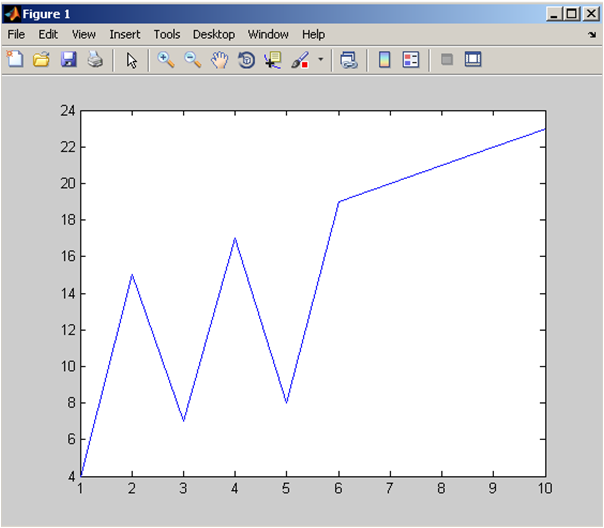
\includegraphics[scale=.75]{figures/matlab_plot1.png}
}\\

Let's take the last example and add some markers and labels.\\

\index{Matlab Functions!\cour{title}}
\index{Matlab Functions!\cour{xlim}}
\index{Matlab Functions!\cour{ylim}}
\index{Matlab Functions!\cour{text}}
\example{ex_labelplot}{\textbf{Plot with labels}\\

\noindent\cour{>> x = [1:10]; y = [4 15 7 17 8 19:23];}\\
\cour{>> plot(x,y,{\color{myred} \textquotesingle-->b\textquotesingle)}}\\
\cour{>> title({\color{myred} \textquotesingle My plot\textquotesingle})}\\
\cour{>> xlim([0,11])}\\
\cour{>> ylim([0,30])}\\
\cour{>> text(7,15,{\color{myred}\textquotesingle My function\textquotesingle})}\\
\\
The plot is now:\\
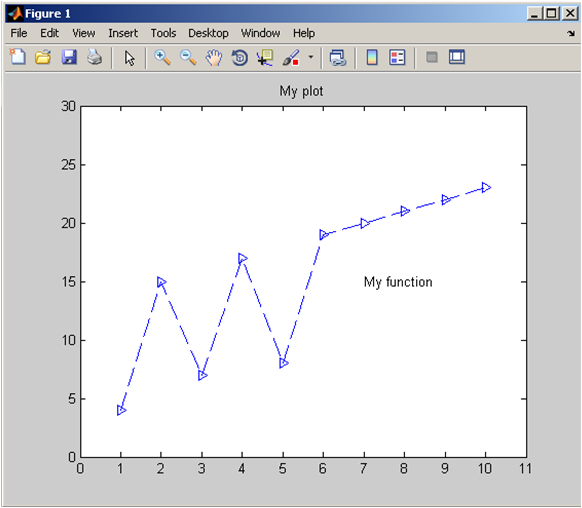
\includegraphics[scale=.75]{figures/matlab_plot2.png}
}\\

In this last example, you can see that there is a title, the limits on the graph are now 0 to 11 (for $x$) and 0 to 30 (for $y$), and there is text on the screen, starting at the coordinate (7,15).  The symbols {\color{myred} \cour{\textquotesingle -->b \textquotesingle}} indicate that the lines should be dashed, the points marked with triangles and the lines colored blue (the default color if none is provided).


If you want to plot more than one set of data in the same figure window, there are two ways to do this.  You can put both in the same \cour{plot} command or by using the \cour{hold} command with two \cour{plot} commands (see next example).\\

\example{ex_twofunctionplot1}{\textbf{Two Functions - one \cour{plot} command}\\

\noindent\cour{>> x1 = [1:10];y1 = [4 15 7 17 8 19:23];}\\
\cour{>> x2 = [3:3:12];y2 = [0 5 3 10];}\\
\cour{>> plot(x1,y1,x2,y2,{\color{myred} \textquotesingle +\textquotesingle})}\\
\cour{>> xlim([0,13]),ylim([-1,25])}\\
\\
The plot is now:\\
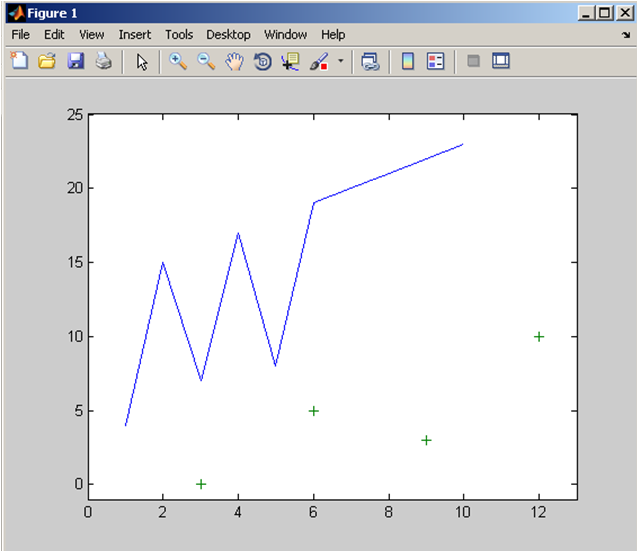
\includegraphics[scale=.75]{figures/matlab_plot3.png}
}\\

So, from this example we can see that if you want to use the same \cour{plot} command, you simply list the pairings, (with any details following each pair) \cour{x1,y1,x2,y2,x3,y3,$\cdots$}.  The default colors start with blue followed by green.  The symbol {\color{myred} \cour{\textquotesingle +\textquotesingle}} means that the second plot is points (not lines) marked with plus signs.\\\\

\index{Matlab Functions!\cour{hold}}
\example{ex_twofunctionplot2}{\textbf{Two Functions - two \cour{plot} commands}\\
\\
We use data from the last example, but use the \cour{hold} command.\\
\\
\cour{>> x1 = [1:10];y1 = [4 15 7 17 8 19:23];}\\
\cour{>> x2 = [3:3:12];y2 = [0 5 3 10];}\\
\cour{>> hold \color{myred} on}\\
\cour{>> plot(x1,y1)}\\
\cour{>> plot(x2,y2,{\color{myred} \textquotesingle +\textquotesingle})}\\
\cour{>> xlim([0,13]),ylim([-1,25])}\\
\\
The plot is now:\\
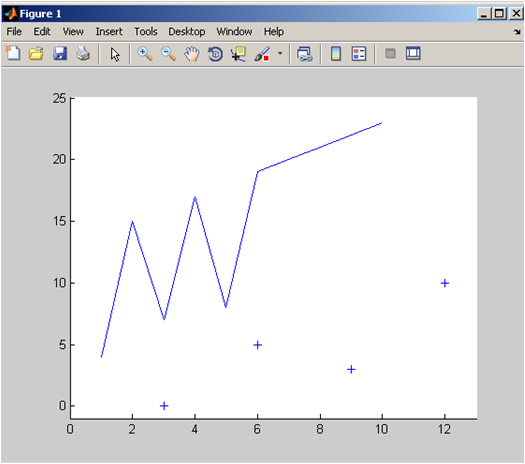
\includegraphics{figures/matlab_plot4.png}
}\\

In the last example, if you didn't include the \cour{hold} command, the second plot would simply overwrite the first.  Also, since we didn't specify new colors, both plots are blue (the default color of a single plot). 

Here we look at the \cour{subplot} command as well as bar graphs and pie charts to create multiple graphs on the same figure.\\

\index{Matlab Functions!\cour{subplot}}
\example{ex_3Dfunctionplot}{\textbf{The \cour{subplot} command}\\
\\
\cour{>> x = [1,2,4,5,8]; y = [x;1:5];}\\
\cour{>> subplot(2,3,1), bar(x)}\\
\cour{>> subplot(2,3,2), bar(y)}\\
\cour{>> subplot(2,3,3), bar3(y)}\\
\cour{>> subplot(2,1,2), pie(x)}\\
\\
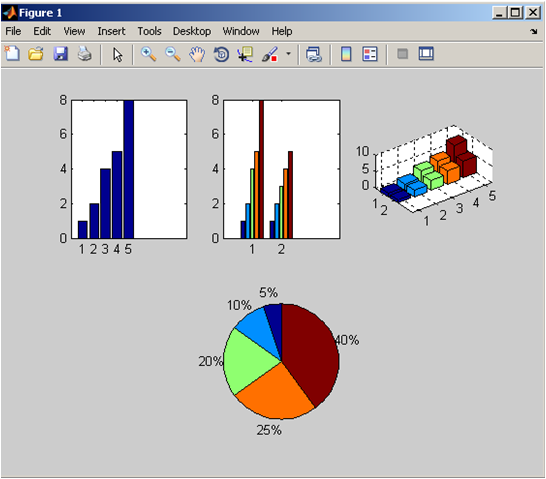
\includegraphics{figures/matlab_plot5.png}

In this example, the \cour{subplot} on each line does two things.  First, it (invisibly) subdivides the figure into rows and columns and second, it indicates where the plot will be shown (counting across the rows).  That is:\\ 
\\
\cour{subplot(\# rows,\# columns, location)}\\

You can see in the example that even though the plot was ``broken up'' into 2 rows and 3 columns in the first three subplot lines, the fourth line re-subdivides the plot into 2 rows and 1 column so that the final plot can take up the entire bottom of the plot.  Using the subplots does not require the \cour{hold} command.}\\

The previous examples give just a beginning of the graphics capabilities of Matlab (including 3D as in the last example).  We will see more graphics in the remainder of the text, but we suggest reading through the help files for (many) more details. 

\newpage
\printexercises{exercises/04_exercises}
%
%Exercises:\\
%For the functions \cour{y = exp(x/5), y = sin(x), y = sqrt(x)} for \cour{x} between 0 and 10:\\
%1) Plot all three on the same plot, but with different colors (use linspace with enough points so that the curves look smooth).  Put in a descriptive title and add text inside the window to label the individual graphs.\\
%2)Plot all three in the same figure window, but with each in their own subplot and each with its own descriptive title.\\






%\definition{def:lineintegral}{\textbf{TITLE}}
%
%\keyidea{idea:lineintprops}{\textbf{TITLE}}
%
%\printexercises{exercises/mathcad_introduction_exercises}
